% !TeX root = ../main.tex
% Add the above to each chapter to make compiling the PDF easier in some editors.

\chapter{Evaluation}\label{chapter:Evaluation}
This chapter is going to demonstrate the functionality of the trained ANN, also it is going to be explained, why there was no part about running the model on Android. After 250000 epochs of training, the NN had an accuracy of 100\% in classifying the validation images correctly, though this result should be treated with caution, as the amount of 39 test images might not be that significant. Furthermore, these pictures did not exhibit any issues regarding the lighting. 

\section{Showcase}\label{sec:showcase}
To present some case to be shown, the related image was chosen to demonstrate "runinference.py" with the related image (Figure: \ref{fig:802}), worth mentioning, the network has never seen this picture before, as it was separated into the validations folder before the actual training began. Running the program with mentioned image results in the output seen in Figure: \ref{fig:programout}. Ignoring the output information about the Tensorflow binary, the output Tensor is printed and it's the eighth score is the highest, fortunately. Additionally, the translation from the highest scoring index to the corresponding image indicates everything went well. 

\begin{figure}[H]
	\centering
	
\includegraphics[width=0.4\linewidth]{images/802(0).jpeg}
	\caption{Test picture 802(0).jpeg}\label{fig:802}
\end{figure}


\begin{figure}[H]
	\centering
	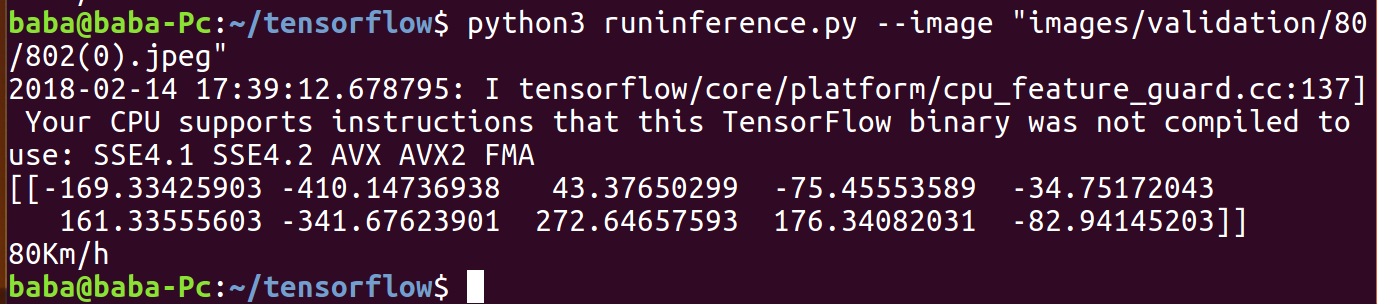
\includegraphics[width=\linewidth]{images/program.png}
	\caption{Test picture 802(0).jpeg}\label{fig:programout}
\end{figure}


\section{Transition to Android}
The classifying phase has been adapted in the Android app and is operable (Figure: \ref{fig:screenfun}). The code is analogue to the version in python (Subsection: \ref{extraction}), but of course, adjusted to Java. 
Unfortunately, due to unforeseeable circumstances, the correct implementation on Android of the Classification. One of the major mistakes was trying the implementation with the NDK, as already mentioned this approach cost about one to two weeks until the decision was made to stop working in that direction. Actually, the task was almost done, it was able to load the model and perform inferences, sadly these requests ended in wrong predictions, therefore with a high probability the mistake lies somewhere in the image extraction or the matrix operations to form a Tensor, in Java. To make matters worse, in a rush, no tool was found to print images when debugging an app in Android Studio. So there is currently no 100 percent accurate or working realization of the demands made in \ref{chapter:Concept}. 
\newline

\begin{figure}[H]
	\centering
	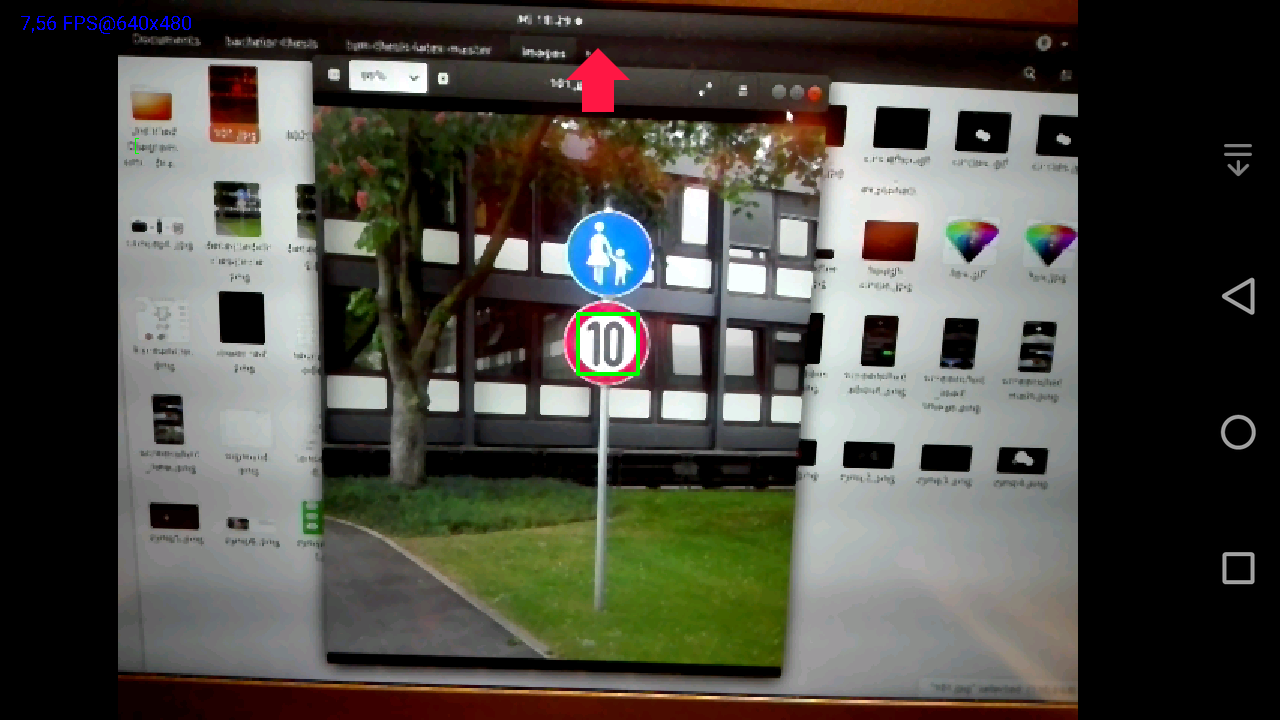
\includegraphics[width=\linewidth]{images/screenshotfun.png}
	\caption{Screenshot of the app running detection on camera mode}\label{fig:screenfun}
\end{figure}